\section{Runner Class Reference}
\label{class_runner}\index{Runner@{Runner}}
Inheritance diagram for Runner::\begin{figure}[H]
\begin{center}
\leavevmode
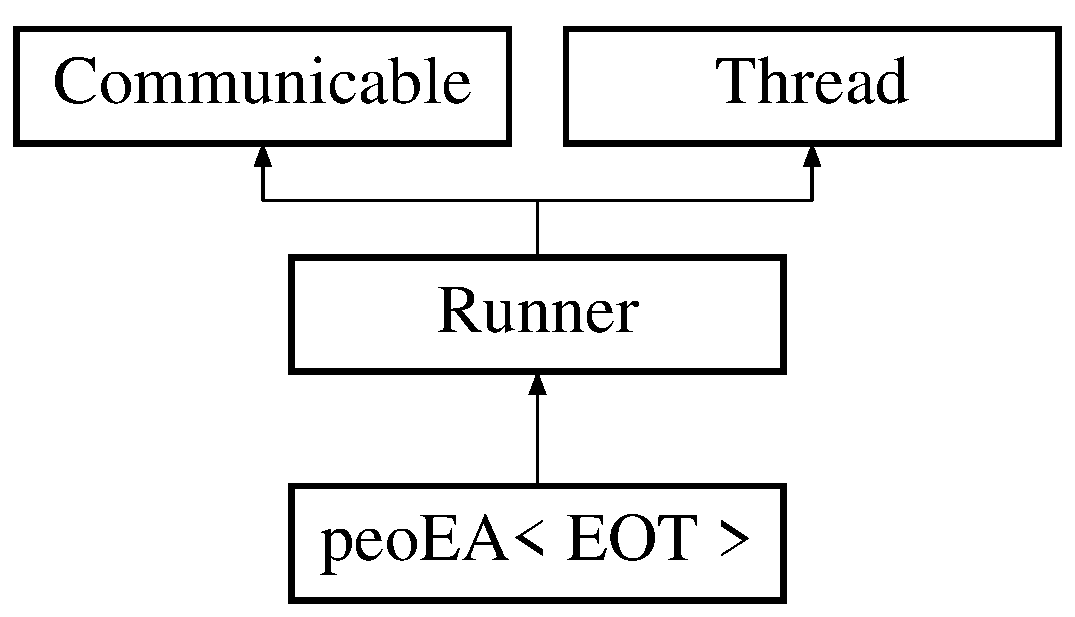
\includegraphics[height=3cm]{class_runner}
\end{center}
\end{figure}
\subsection*{Public Member Functions}
\begin{CompactItemize}
\item 
{\bf Runner} ()\label{class_runner_7acb8258c21da9daa62f9a177a2e5acd}

\item 
void {\bf start} ()\label{class_runner_7dc4419051fcc5cc9dadd54ecc9cd47d}

\item 
void {\bf wait\-Starting} ()\label{class_runner_5bc239db2be753b77369fa9a038769fd}

\item 
bool {\bf is\-Local} ()\label{class_runner_40adbfb7d6944189b4fff60b02e669ca}

\item 
void {\bf terminate} ()\label{class_runner_0f133e75c28fb8264549814f80608e68}

\item 
virtual void {\bf run} ()=0\label{class_runner_2d306c1835d8710258d2b52b8cc8312c}

\item 
RUNNER\_\-ID {\bf get\-ID} ()\label{class_runner_5026c74eec184e3a15cb3c0ec4200a57}

\item 
void {\bf pack\-Termination} ()\label{class_runner_2ad6d199d684d6f34347fc202ffe2fa3}

\item 
void {\bf notify\-Sending\-Termination} ()\label{class_runner_3591be473e0fcee1105fb57319b529aa}

\end{CompactItemize}
\subsection*{Private Attributes}
\begin{CompactItemize}
\item 
sem\_\-t {\bf sem\_\-start}\label{class_runner_4b0827d5df2df632db4ab71dd55e81b2}

\item 
unsigned {\bf id}\label{class_runner_1989c1f8e0b0b54ad2e60a341007e59d}

\end{CompactItemize}


\subsection{Detailed Description}




Definition at line 34 of file runner.h.

The documentation for this class was generated from the following files:\begin{CompactItemize}
\item 
runner.h\item 
core/runner.cpp\item 
rmc/mpi/runner.cpp\end{CompactItemize}
